\chapter{Provvedimenti attuati e Best-Practice}
\label{chap:best_p}

Il presente capitolo ha lo scopo di ripercorrere la storia recente del Secondary Ticketing per scoprire i maggiori provvedimenti attuati e le varie tipologie di azioni intraprese. 
Si vuole inoltre concentrare l'attenzione sull'efficacia di tali accorgimenti: una tale analisi potrà essere utile in futuro per futuri investimenti nel tentativo di arginare il fenomeno del Secondary Ticketing. 
Sono state individuate tre macro-categorie, utili per la classificazione: 
\begin{itemize}
\item \textit{\textbf{Provvedimenti Legali}}: emendamenti e leggi emanate per contrastare il fenomeno, descritti nella Sezione \ref{sec:legal}
\item \textit{\textbf{Provvedimenti Strategici}}: azioni strategiche intraprese dalle aziende coinvolte, descritti nella Sezione \ref{sec:strat}
\item \textit{\textbf{Provvedimenti Tecnici}}: accorgimenti a livello software e modifiche del sistema di vendita, descritti nella Sezione \ref{sec:tech}
\end{itemize}

\section{Provvedimenti Legali} \label{sec:legal}
Si è a lungo pensato che un rafforzamento delle leggi contrastanti il Secondary Ticketing, unito a controlli più rigidi e scrupolosi delle autorità competenti, fosse la strategia chiave da seguire e in cui investire tempo e risorse. 
L'assenza di una unica Legge Federale, valida per una moltitudine di paesi, è stata a lungo additata come l'unica soluzione possibile al problema: numerose e pesanti però sono state le opposizioni a un simile emendamento, sia da parte dei rivenditori primari che di quelli secondari, come nota Drayer (\cite{drayer2011examining}).
Sono numerosi tuttora i casi in cui i portali di Secondary Ticketing non seguono le direttive imposte dal Codice di Condotta redatto dall'associazione europea "EU Secondary Ticketing Association" (EUSTA), con sede in Olanda (\cite{phdthesis}). 
La località delle leggi è un altro problema degno di menzione: infatti, con lo sviluppo e l'attuale prevalenza della rivendita tramite siti web dedicati, molte vendite non sono assegnabili ad alcuna giurisdizione, e pertanto non risultano perseguibili a livello legale. 
Drayer inoltre evidenzia come la tendenza verso la deregolamentazione e la legittimazione del mercato secondario sia sempre più netta: sono numerosi infatti gli Stati ad aver abolito le precedenti regolamentazioni contro il Secondary Ticketing, in particolare negli Stati Uniti e nei paradisi fiscali. 
Nel dicembre del 2016 è stato approvato il cosiddetto "\textit{\textbf{BOTS Act}}" (\textit{Better Online Ticket Sales}), legge federale che rende reato penale l'uso di software in grado di aggirare le misure di sicurezza dei siti di e-commerce al fine di acquistare ingenti quantità di titoli di accesso. Il decreto rende inoltre obbligatori diversi accorgimenti che tutti i portali di Secondary Ticketing dovranno adottare: il più rilevante è la segnalazione chiara della natura del portale nella pagina principale. 
Sono molte, infatti, le lamentele pervenute da utenti ingannati dall'aspetto dei portali di Secondary Ticketing: un caso rilevante è quello nato in seguito al concerto dei Queen a Bologna nel novembre del 2017, in cui molti clienti si lamentarono presso il promoter per aver pagato un prezzo nettamente superiore al "face value".
La sottile differenza tra i portali primari e secondari è mostrata nelle seguenti immagini: da una parte il rivenditore ufficiale TicketOne (Figura \ref{ticketone}), dall'altra il rivenditore Viagogo (Figura \ref{viagogo}).
\begin{figure}[htbp]
	\centering
	
\includegraphics[width=0.68\textwidth]{chapter3/immagini/ticketone_1}
	\caption{TicketOne}
	\label{ticketone}
\end{figure}
\begin{figure}[htbp]
	\centering
	
\includegraphics[width=0.68\textwidth]{chapter3/immagini/viagogo_disclaimer}
	\caption{Viagogo}
	\label{viagogo}
\end{figure}
Lo stesso Drayer ha inoltre condotto diverse interviste ad agenti di polizia statiunitensi per ricevere informazioni riguardo al trattamento del Secondary Ticketing da parte delle autorità: da queste conversazioni emerge il fatto che venga fatta molta più attenzione ai biglietti rubati o contraffatti, piuttosto che alla rivendita dilagante: il reato di truffa e/o di contraffazione è infatti considerato più grave e degno di pene esemplari, oltre che più semplice da riconoscere. La tendenza emersa in seguito a queste interviste con le autorità  statunitensi è quella di considerare la pratica del bagarinaggio usuale e meno pericolosa di reati come frode o contraffazione. 

\section{Provvedimenti Strategici} \label{sec:strat}
In questa sezione verranno discusse le azioni intraprese dagli agenti coinvolti a livello di business: cambiamenti di strategia, accordi commerciali, accettazione o rifiuto del Secondary Ticketing. 
\subsection {Provvedimenti Collaborativi}
Molte aziende coinvolte, tra cui società sportive, promoter di eventi e talvolta direttamente gli artisti, hanno scelto di stringere accordi di collaborazione coi portali di Secondary Ticketing. Non è infrequente infatti vedere che molti club appartenenti alle leghe sportive più famose globalmente hanno pagine dedicate su tali portali. Una tale scelta si giustifica per i seguenti motivi: 
\begin{itemize}
\item Così facendo, la società si assicura la possibilità di "ricatturare" parte del surplus riservato al consumatore e inoltre riduce i guadagni degli speculatori.
\item La creazione di un canale di vendita secondario ufficiale riduce drasticamente la quantità di biglietti contraffatti, in quanto ogni titolo di accesso viene preventivamente validato per la rivendita \cite{shapiro2014examination}.
\end{itemize}
In questo caso la progressiva deregolamentazione viene affiancata da un tentativo di legittimazione del mercato e di protezione del consumatore finale. L'opinione comune in questo ambito è che sia più semplice accettare il Secondary Ticketing e renderlo parte integrante del proprio operato piuttosto che escogitare strategie e soluzioni in grado di combatterlo \cite{simon2003if}, in quanto i vantaggi a livello economico sono più ingenti rispetto a una lunga e continua politica di ricerca e sviluppo. 
Un approccio simile risolve però un problema fondamentale, da sempre una piaga al pari della speculazione, ovvero rimuove quasi del tutto il rischio di truffa e contraffazione, in quanto i titoli di accesso, seppur venduti su portali secondari, sono validati e controllati dalla società che li ha emessi sul mercato. 
%Inserire screenshot da StubHub
\begin{figure}[H]
	\centering
	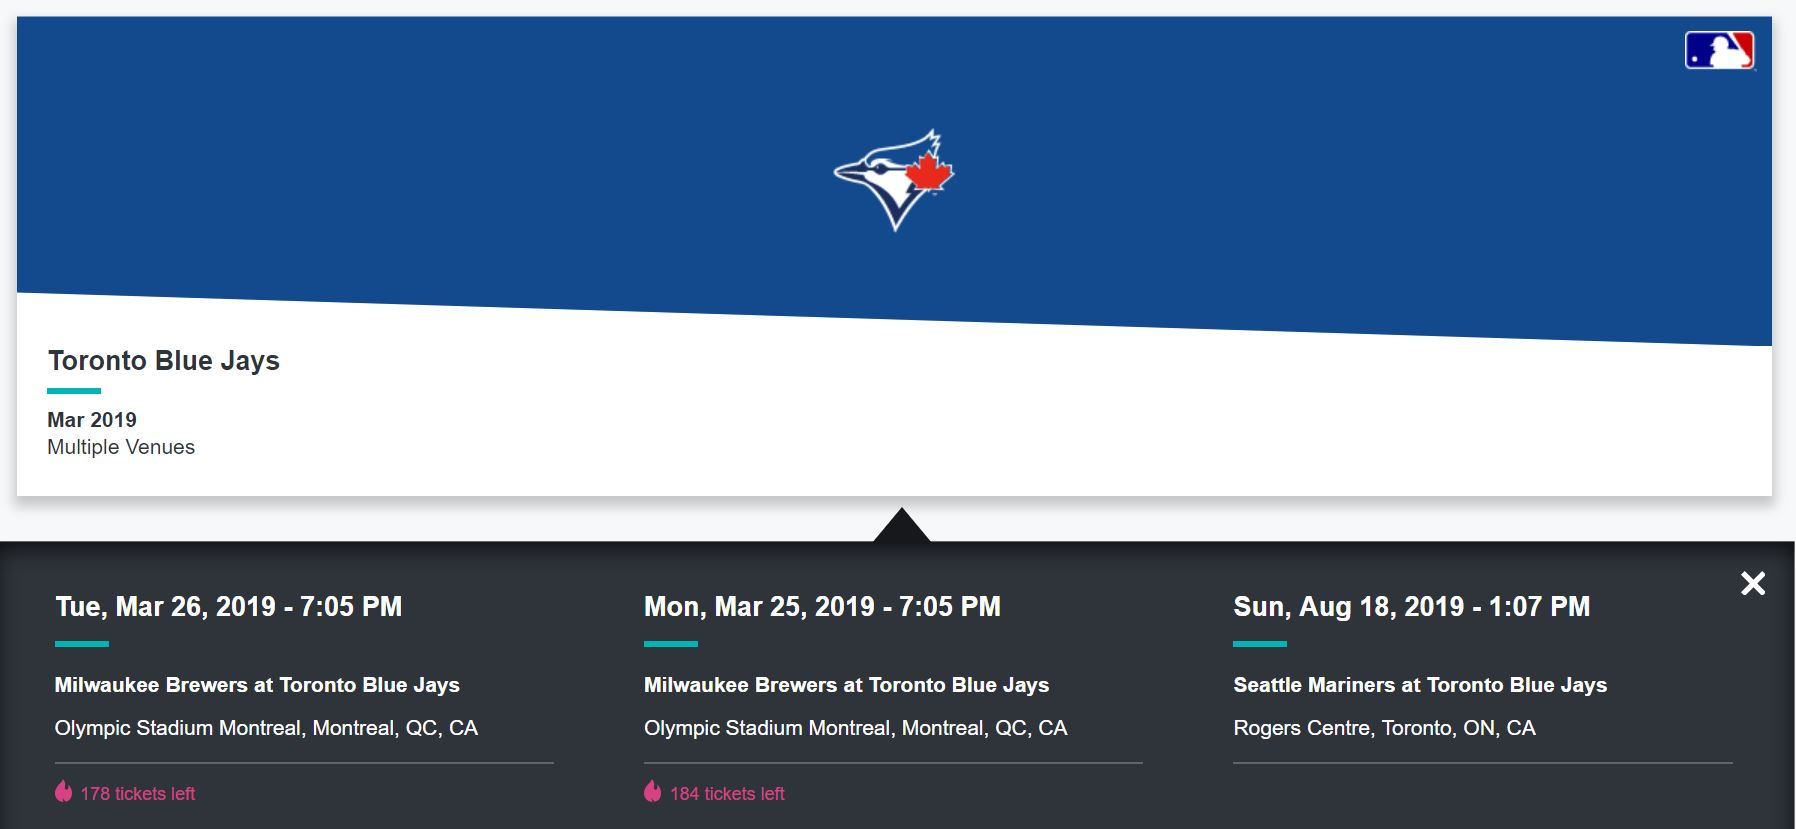
\includegraphics[width=0.68\textwidth]{chapter3/immagini/StubHub_Club}
	\caption{StubHub e le partnership con le società sportive}
	\label{stubhub_part}
\end{figure}
I recenti provvedimenti intrapresi dalle principali società di Ticketing puntano verso l'integrazione dei sistemi di rivendita all'interno dei portali di vendita primaria: così facendo, il risultato sarebbe quello di ottenere un unico portale integrato effettuando una cosiddetta \textit{estensione di linea}. La prima società a riuscire nell'intento è stata TicketMaster, che a fine 2018 ha sviluppato la piattaforma \textit{TicketExchange} (Figura \ref{exc}) raggiungibile proprio dal portale primario. Il portale tratta la rivendita di biglietti per diversi tipi di manifestazione e ha accordi commerciali con diverse leghe sportive statunitensi. Ad ora, TicketExchange non è disponibile in Italia. 
\begin{figure}[htbp]
	\centering
	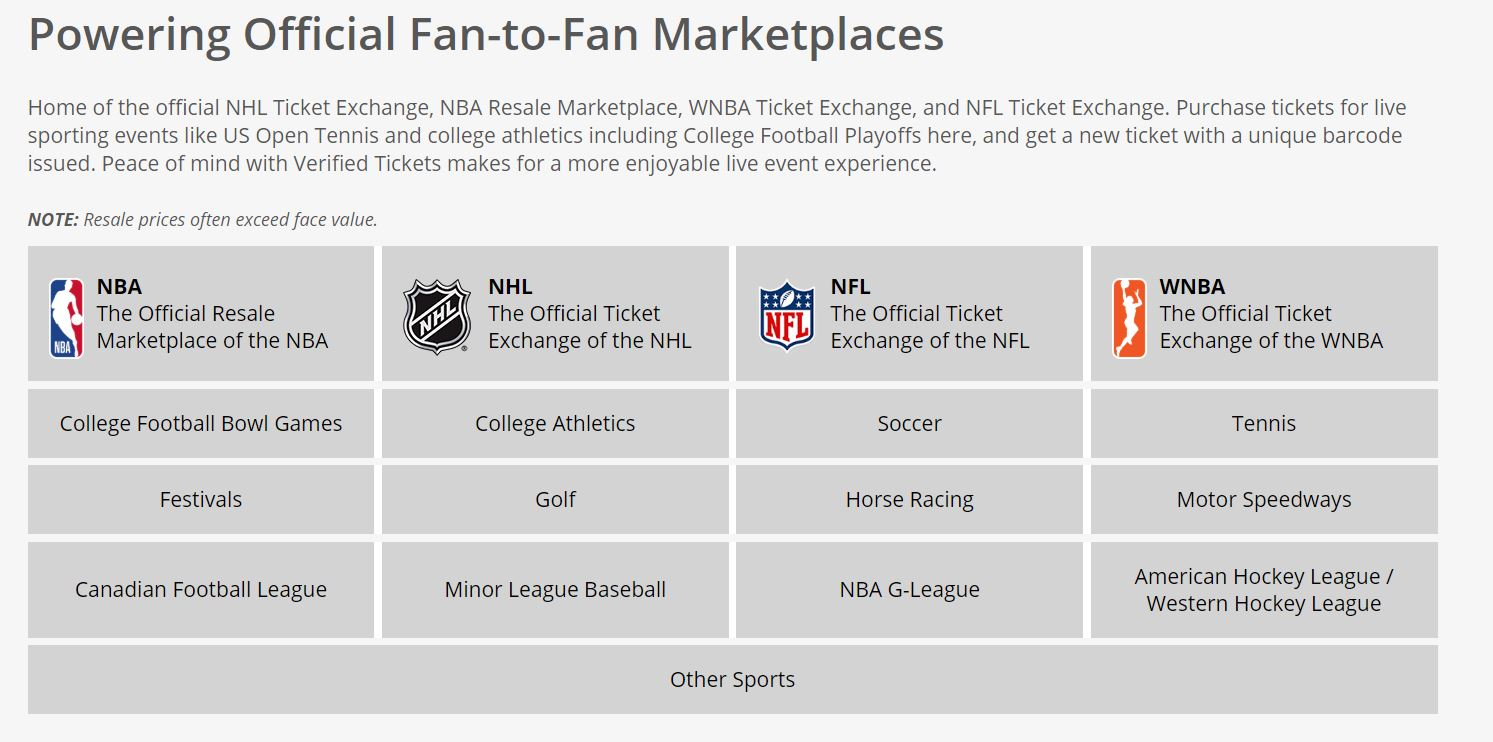
\includegraphics[width=0.68\textwidth]{chapter3/immagini/exchange}
	\caption{Pagina princiale del sito \textit{TicketExchange by Ticketmaster}}
	\label{exc}
\end{figure}
\subsection{Provvedimenti di contenimento}
Se da una parte alcuni agenti scelgono di collaborare con gli enti secondari, ci sono altrettanti casi di aziende determinate a combattere il fenomeno. Tra queste si annoverano in particolare i sistemi di biglietteria e i promoter. 
Verranno ora discussi i principali provvedimenti di contenimento del fenomeno, con relativi risultati. 
Di particolare interesse è notare che i provvedimenti strategici impattanti sulle politiche di pricing e distribuzione dei titoli di accesso si siano dimostrati più performanti da un punto di vista di contenimento del fenomeno, in quanto modificano drasticamente la struttura del mercato. 
\subsubsection{Ticket Pricing Dinamico} \label{dtp}
L'avvento del Secondary Ticketing "digitale" ha avuto un impatto notevole sulle politiche di pricing dei biglietti, che notoriamente, hanno un valore di emissione molto inferiore al valore di mercato. (\cite{courty2014pricing})
Intorno ai primi anni 2000 la mancanza di differenziazione di presso tra i titoli di accesso era additata come la maggiore causa di speculazioni da parte di agenti secondari, da lì l'adozione di politiche di Variable Ticket Pricing (\textit{VTP}), ovvero logiche di pricing ("\textit{Price Discrimination}")che mirano a differenziare la qualità dei posti in base al tipo di venue e all'esclusività dell'evento. 
Successivamente sono stati progettati degli algoritmi che variano dinamicamente il prezzo del biglietto in base alla domanda del consumatore e una serie di variabili indipendenti. Tale tecnica è definita come Dynamic Ticket Pricing (\textit{DTP}), ed è da tempo adottata da compagnie aeree e strutture alberghiere.
Nell'ambito degli eventi, sportivi o artistici, nell'algoritmo predittivo di prezzo e domanda vengono considerate molte variabili rispetto al settore dei servizi, e si tratta in particolare non solo di variabili inerenti all'evento nella sua unicità, ma anche a fattori esogeni come meteo, orario o una particolare situazione nella città che ospiterà l'evento. 
Sebbene gli algoritmi di DTP rappresentino la normalità nell'ambito del settore dei servizi da almeno vent'anni, occorre precisare che, nell'ambito delle manifestazioni sportive, le prime implementazioni risalgono soltanto al 2007, quando la squadra NFL dei San Francisco Giants sperimentò questa soluzione per la vendita di tutti i biglietti non riservati agli abbonati \cite{article}. Nel mondo della musica sono invece più rari gli episodi di concerti/eventi in cui i tutti i titoli di accesso siano stati venduti con prezzo variabile (fanno eccezione, tra gli altri, i recenti tour di Taylor Swift e Jay-Z \cite{swiftrs}): è più comune il fatto che vengano venduti con prezzo dinamico solo i cosiddetti "biglietti VIP", che includono numerosi benefit in aggiunta all'evento, tra cui ingressi prioritari, catering riservato, oggetti ricordo e/o incontri con l'artista. 
Nel mondo della musica si predilige invece la politica di Price Discrimination, ma è possibile osservare con buona frequenza eventi in cui tutti i biglietti hanno un solo prezzo fissato \cite{courty2011unpriced, eckard2013impact}. 
Le variabili più rilevanti per gli algoritmi di pricing dinamico (DTP), come fa notare Shapiro \cite{shapiro2014examination}, sono: 
\begin{itemize}
\item Data dell'evento, in particolare il giorno della settimana;
\item Orario della manifestazione;
\item Trend delle squadre partecipanti; (in caso di evento sportivo)
\item Parte della stagione sportiva: ad esempio, una partita di una fase eliminatoria genera più interesse di una partita di campionato, che non necessariamente può essere utile ai fini della classifica;
\item Interesse ("\textit{buzz}" o "\textit{hype}") per l'evento, misurato tramite le interazioni degli utenti sui social media \cite{o2018hashmoney} e la domanda effettiva registrata;
\item Unicità dell'evento: è determinante sapere se l'evento è parte, ad esempio, di una fase ad eliminazione diretta, o, in un altro settore, se per caso si tratta di una data unica di un tour promozionale, piuttosto che sapere se si tratti di un evento ripetuto lungo un dato arco temporale;
\item Meteo.
\end{itemize}
Gli algoritmi di DTP possono variare in base alla politica di \textit{Revenue Management} \cite{drayer2012dynamic} dell'azienda e al mercato in cui essa è posizionata. Basandosi sulle analisi di mercato disponibili, emerge che aziende come compagnie aeree e alberghiere, operanti nel settore dei servizi, tendano ad adottare politiche di \textit{Revenue Maximization}, volte ad aumentare i guadagni tramite politiche di pricing aggressive e vendita di beni complementari, in modo da cattuare quanto più possibile dal consumatore finale, in termini di liquidità. Il settore degli eventi presenta invece maggiori vincoli dal punto di vista strategico e organizzativo: si pensi, per esempio, alla necessità di dover puntare sempre al riempimento della venue il giorno dell'evento, oppure alla volontà di puntare sul benessere psicologico e sulla soddisfazione del cliente, che così potrà sentirsi felice e iniziare una collaborazione economica con l'organizzazione. Queste differenze sostanziali, unite a quelle descritte nel Capitolo \ref{chap:stato_arte}, sono le ragioni per cui in questo settore vengono preferite strategie di \textit{Attendance Maximization}, che puntano su prezzi più competitivi e sul benessere psicofisico del consumatore. In questo scenario si pone particolare attenzione ai guadagni derivanti dalla vendita dei cosiddetti \textit{Complementary Goods} e dalle collaborazioni di ordine pubblicitario, piuttosto che concentrare la ricerca di guadagno sulla vendita dei titoli di accesso \cite{drayer2012dynamic}.
Così facendo, i prezzi si allineano con la domanda del consumatore e arrivano ad assumere valori vicini al loro reale valore di mercato, riducendo la possibilità, per gli speculatori, di catturare il surplus del consumatore.
Questa soluzione finora è stata quella più efficiente, in termini di riduzione del fenomeno di Secondary Ticketing per gli eventi coinvolti \cite{loewenstein2010ticket}: è stato infatti stimato che l'applicazione della differenziazione di prezzo (\textit{Price Discrimination}) porta a guadagni mediamente maggiori del 5\% rispetto all'applicazione di un singolo prezzo per tutti i titoli di accesso (\cite{courty2012impact}). 

\subsubsection{Paperless Ticket}
L'eliminazione del biglietto cartaceo, facilmente trasferibile, in favore di uno digitale, strettamente nominale, a cui accompagnare documento di riconoscimento e carta di credito, si è dimostrata una soluzione estremamente efficiente per il contenimento dei bot automatizzati. L'impossibilità di acquistare biglietti anonimi distoglie l'interesse dello speculatore, in quanto la possibilità di un'eventuale rivendita è prossima allo zero.
Numerosi artisti hanno scelto di abbracciare questa logica di distribuzione, tra cui Tom Waits, AC/DC, Metallica e Miley Cyrus, con risultati positivi (\cite{drayer2011examining}).
\paragraph{Biglietti nominali in Italia}
Il 26 novembre 2018 in Italia è stato approvato un emendamento alla legge di bilancio che si prepone lo scopo di arginare il fenomeno del Secondary Ticketing: dal 1/07/2019 sarà infatti obbligatorio emettere biglietto nominale per tutti gli eventi situati in luoghi la cui capienza è uguale o maggiore di 5.000 persone \cite{larepbag}. Nell'emendamento sarebbe inoltre inclusa la possibilità di poter rivendere il proprio biglietto nominale soltanto tramite piattaforme ufficiali che dispongano di una tecnologia certificata per il cambio del nominativo del titolo di accesso: il problema, ad oggi, è insito nel fatto che al momento tale piattaforma non esiste sul territorio italiano e non si hanno aggiornamenti riguardo a sviluppi da parte dei principali portali, come Ticketone e Ticketmaster.
Il processo descritto nell'emendamento prevede che la rivendita del biglietto nominale possa avvenire soltanto nella seguente maniera: 
\begin{enumerate}
\item L'utente rimette in vendita il proprio biglietto sul portale pagando una commissione.
\item Il possibile compratore acquista il biglietto pagando prezzo del biglietto e dovute commissioni.
\item Il biglietto appartenente al precedente proprietario perde ogni validità e ne viene emesso un altro per lo stesso posto a nome del nuovo compratore. 
\end{enumerate}   
Questo provvedimento è stato a lungo osteggiato dalle più grosse società agenti nel mercato del Ticketing, in particolare da Live Nation e Ticketone (e in generale il gruppo Cts Eventim) \cite{solebag}. Le principali critiche mosse sono le seguenti: 
\begin{itemize}
\item Il provvedimento vieta qualsiasi tipo di scambi tra privati senza passare dalla piattaforma adibita. Questo comporta costi maggiori per entrambi gli attori coinvolti nella transazione. 
\item Il provvedimento limita la libertà dell'acquirente, in quanto verrebbe totalmente esclusa l'eventualità di comprare biglietti per regalo o con largo anticipo per assicurarsi la partecipazione.
\item Aumenterebbero i costi di organizzazione (es. gestione delle code, maggiore personale per controlli ecc.), che ricadrebbero sul prezzo del biglietto, già in costante aumento come meccanismo di risposta al dilagante bagarinaggio. 
\item Il provvedimento non prevede alcun aumento delle multe o di controlli nei confronti del Secondary Ticketing online, sebbene al momento esistano già delle leggi adibite. 
\end{itemize}

\paragraph{Verified Fan Program} 
Il \textit{Verified Fan Program}, sviluppato da TicketMaster in collaborazione con gli artisti aderenti, consiste in una nuova procedura informatica che si pone l'obiettivo di effettuare una scrematura preliminare tra bot e persone fisiche realmente interessate all'evento. \\Ogni artista ha un programma dedicato, e un utente può registrarsi gratuitamente a tale programma fornendo i suoi dati. Il sistema, tramite un algoritmo proprietario e l'uso di una Intelligenza Artificiale, verifica la "`legittimità"' dell'utente e ne valida l'ingresso al programma. Gli utenti iscritti al programma entro una certa data avranno accesso a una vendita anticipata dei biglietti tramite una lotteria: una percentuale di queste persone verrà estratta per poter acquistare un biglietto prima della messa in vendita per il pubblico. \\TicketMaster stima che, dei biglietti venduti tramite il Verified Fan Program, solo una percentuale tra il 3 e il 5\% sia stata rivenduta sui portali secondari. 
Diversi artisti hanno adottato questo programma, tra cui \textit{U2}, \textit{Bruce Springsteen}, \textit{Anderson .Paak}, \textit{Taylor Swift}, \textit{Vampire Weekend} e \textit{Elton John}.

\subsubsection{Aumento dei prezzi}
L'aumento dei prezzi dei biglietti (si stima che tra il 2005 e il 2017 l'incremento medio sia circa dell'88\%, \cite{tompkins2018ticket}) è una misura fisiologica nel tentativo di contrastare il fenomeno del Secondary Ticketing. Nonostante i cospicui innalzamenti di prezzo, non sempre questa politica si è rivelata efficace come deterrente dalla speculazione, probabilmente perché, nonostante l'aumento, il prezzo effettivo dei biglietti era ancora troppo basso rispetto al reale valore di mercato. 
Una tecnica comune per comprendere al meglio come prezzare i propri biglietti è osservare i trend delle vendite sul mercato secondario per quanto riguarda l'artista o l'evento in questione nelle precedenti occasioni, per poi scegliere un prezzo che non sia distante dal prezzo medio delle vendite "non ufficiali" \cite{tompkins2018ticket, courty2014pricing}.
Si annoverano pochi casi in cui un aumento ingente dei prezzi ha veramente fatto sì che non vi fosse mercato per gli speculatori, in quanto valore di emissione e valore di mercato avevano verosimilmente lo stesso valore. Recenti esempio sono il "\textit{Reputation Tour}" di \textit{Taylor Swift} negli stadi statiunitensi, e il "\textit{4:44 Tour}" del rapper \textit{Jay-Z} (Forbes, 2018). Una tale scelta si discosta dalla classica visione che tende a quantificare il successo di un tour con le vendite "istantanee" dei biglietti. 
La vendita graduale dei titoli, le bassissime percentuali di biglietti sul mercato secondario (Si stima siano state intorno al 5\%, di cui una parte a prezzi molto inferiori del valore di emissione) hanno invece rappresentato una svolta nella lotta al Secondary Ticketing. 
Non sempre però un'alternativa simile è attuabile: per molti enti o artisti una politica di consistente aumento dei prezzi rappresenterebbe un possibile, irreparabile danno di immagine. 
%possibile digressione sulle ragioni
Per artisti affiliati a etichette discografiche indipendenti, con un bacino di utenza di ascoltatori minore e meno possibilità di usufruire di passaggi in radio e pubblicità tramite mezzi di comunicazione digitali, il cui successo si basa principalmente su una nicchia di ascoltatori, collezionisti di dischi e frequentatori di concerti, una politica di aumento cospicuo del prezzo potrebbe risultare fatale, perché essa avrebbe impatto sulle vendite del merchandising (che rischiano di calare) e riscuoterebbe un effetto negativo sul pubblico, che percepirebbe un maggiore distacco in favore di un mero rientro finanziario. 

%\subsubsubsection{Ticketmaster: un caso unico}

\section{Provvedimenti Tecnici} \label{sec:tech}
Questa sezione descrive i maggiori provvedimenti attuati dal punto di vista informatico, con relativi risultati.
\subsection{CAPTCHA} \label{captcha}
L'acronimo CAPTCHA ("\textbf{C}ompletely \textbf{A}utomated \textbf{P}ublic \textbf{T}uring-test-to-tell \textbf{C}omputers and \textbf{H}umans \textbf{A}part") indica un particolare test di Turing, sviluppato nel 2003 da un gruppo di ricercatori capeggiati da Van Ahn \cite{von2003captcha}, atto a scoprire se l'utente testato è un essere umano oppure un computer (in particolare, un bot). Tale test, progettato in modo da essere superato facilmente da un umano, ma al contempo da essere insuperabile per un computer, consiste nel riconoscimento di una stringa di testo all'interno di un'immagine, nel riconoscimento di foto contenenti determinati oggetti: azioni usuali per una persona fisica, ma teoricamente impossibili per un calcolatore automatizzato. 
L'introduzione dei CAPTCHA nella  maggioranza dei siti web è stata in grado di ridurre drasticamente la creazione automatizzata di indirizzi e-mail ai fini di spam, evitare lo screening da parte dei "search engine bots" per i siti che non lo desiderino e migliorare la comunicazione tra utenti, in particolare nei forum e nelle pagine di customer service.
%Immagine captcha
\begin{figure}[H]
	\centering
	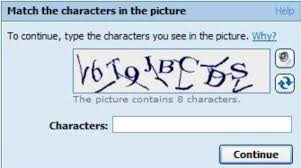
\includegraphics[width=0.68\textwidth]{chapter3/immagini/captcha}
	\caption{Tipico esempio di CAPTCHA}
	\label{captcha}
\end{figure}
\subsubsection{Inefficacia del CAPTCHA nel mondo del ticketing}
\`E stato dimostrato che i ticket bot sono in grado di eludere la misura di sicurezza rappresentata dal CAPTCHA tramite software di image matching che sfruttano la staticità delle immagini del sistema CAPTCHA.
In numerosi casi i bot si sono dimostrati capaci di eludere la misura di sicurezza elaborata dal CAPTCHA: stando a quanto rivelato da \textit{Kenneth Lowson} \cite{vicelowson}, inventore dei ticket bot (un'immagine dell'interfaccia è mostrata in Figura \ref{bot1}) ed ex titolare dell'agenzia di Secondary Ticketing \textit{Wiseguy Tickets} fino al 2010, anno in cui Lowson e collaboratori furono arrestati con l'accusa di truffa e violazione di sistema informatico, il database di immagini CAPTCHA è statico e contiene circa 30.000 immagini. Lowson e i suoi collaboratori si cimentarono nell'impresa di scaricare localmente ogni singola immagine della base di dati, per poi associarla univocamente con la stringa di testo in grado di risolvere di un problema, piuttosto che ricorrere al algoritmi di Machine Learning, decisamente meno performanti in questo ambito. 
\begin{figure}[H]
	\centering
	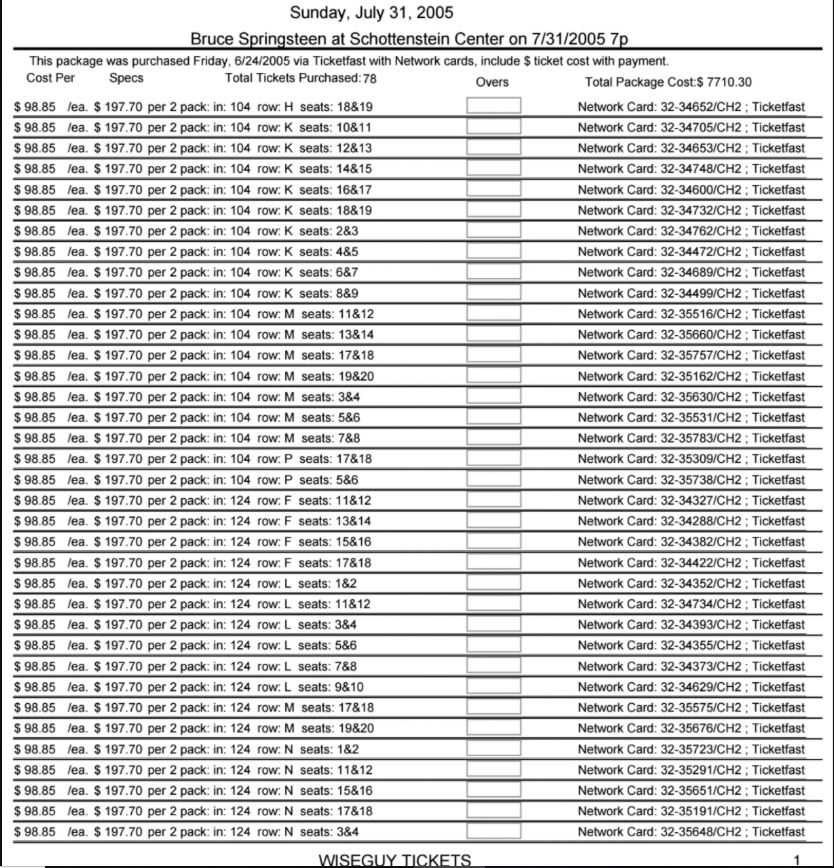
\includegraphics[width=0.68\textwidth, height=20cm]{chapter4/immagini/bot1}
	\caption{Screenshot del bot creato da Lowson}
	\label{bot1}
\end{figure} 
\'E stato inoltre condotto un esperimento nel 2007 che ha dimostrato l'inefficacia del protocollo CAPTCHA nei siti adibiti al ticketing \cite{caine2007ai}: tale test si basava su ripetute richieste al server addetto alla generazione delle immagini. Dalla ricerca emerse che il server, se sollecitato, rispondeva all'utente fornendo immagini simili tra loro, semplici da decifrare per un bot tramite prima un algoritmo "\emph{k-means}" e poi una cross-correlazione normalizzata \cite{dimicco2001dynamic}. 
L'esperimento era così articolato: 
\begin{enumerate}
\item Download di un numero sufficienti di immagini di CAPTCHA
\item Ottenimento di un cosiddetto \textit{Template}, ovvero un elenco di tutti i caratteri utilizzati dal CAPTCHA pulito da ogni forma di rumore grafico
\item segmentazione dell'immagine del CAPTCHA tramite l'algoritmo k-means
\item Utilizzo della cross-correlazione ogni volta che un carattere viene paragonato a un'immagine target. L'algoritmo assegna un punteggio $S$ in base all'immagine con la quale il carattere esaminato viene confrontato.
\end{enumerate}
I risultati del test confermarono che il bot preso in esame (sviluppato dagli autori dell'articolo) fu in grado di violare il CAPTCHA del sito \textit{tickets.com} 40 volte su 40, con un tempo medio di 9.89 secondi e 7.2 interrogazioni al database di CAPTCHA, contro i 60 concessi dal firewall del sito per il completamento del CAPTCHA daparte di un essere umano.
%\subsection{Verified Fan Program}
\subsection{CitizenTicket e la blockchain BitTicket} \label{block}
Nel 2017, il portale di vendita biglietti Citizen Ticket, con sede a Londra, sviluppa \emph{BitTicket}, basata sulla Virtual Machine Ethereum, la prima \textbf{\textit{blockchain}} adibita esclusivamente alla vendita dei titoli di accesso, con l'intento di combattere l'uso massiccio dei bot. 
Per blockchain si intende una struttura dati condivisa e immutabile, ed è assimilabile a una base di dati distribuita, in cui ogni \textit{nodo} ha una copia privata dei dati. Data la particolare struttura della blockchain, tutti i nodi hanno lo stesso livello di affidabilità e ciascuno di essi è protetto da crittografia con chiave pubblica. 
La possibilità di creare una biglietteria online basata su blockchain è già stata discussa negli ultimi anni nella letteratura scientifica \cite{tackmann2017secure} e, per quanto poi questa idea non sia stata ancora dovutamente approfondita, potrebbe rappresentare una potenziale rivoluzione nella gestione dei titoli di accesso. 
Ogni nodo della blockchain è univocamente identificato dai seguenti parametri, specificati nell'\textit{header}: 
\begin{itemize}
\item \textbf{\textit{Versione}}: indica il software utilizzato
\item \textbf{\textit{PrevHash}}: hash di 256 bit che fa riferimento all'Hash del blocco precedente
\item \textbf{\textit{Merkle Root}}: hash che indica tutti i blocchi del gruppo
\item \textbf{\textit{Timestamp}}: indicatore temporale della transazione
\end{itemize}
La differenza principale tra blockchain e base di dati distribuita risiede nel fatto che l'aggiunta alla blockchain di un nuovo nodo, o la registrazione di una qualsiasi transazione, necessitino di un'approvazione e di una validazione ("\textbf{\textit{mining}}") da parte di un sottoinsieme ristretto di blocchi adibiti a questa funzione.  
La natura intrinsecamente distribuita della blockchain fa sì che la transazione non venga istantaneamente validata e approvata da una base di dati centrale, e pertanto contrasta il concetto di bulk buy: se ogni transazione necessita di approvazioni da un numero di nodi maggiore di 1, la velocità di acquisto dei bot sarà notevolmente diminuita, e la loro identità sarà facilmente individuabile.
Grazie a una simile implementazione, sarebbe tracciabile il ciclo di vita di ogni singolo biglietto venduto sulla blockchain, e sarebbe possibile riconoscere subito pattern di acquisto anomali e annullare le transazioni in risposta. \\
Per la realizzazione di una biglietteria con blockchain, Tackmann \cite{tackmann2017secure}, ricercatore IBM, propone una soluzione basata su \emph{Hyperledger Fabric}, software open source sviluppato dalla Linux Foundation in collaborazione con numerose aziende informatiche (tra cui, ad esempio, SAP e IBM) a partire dal 2015 per la creazione e la gestione di blockchain. La soluzione proposta è una biglietteria basata su blockchain e "\textit{Smart Contract}". \\ 
Per Smart Contract si intende uno script salvato su ogni nodo della blockchain, che viene azionato ed eseguito in seguito ad un "Trigger" che ne richiede l'esecuzione \cite{christidis2016blockchains}. Il contratto viene eseguito da ogni nodo della blockchain con i dati in ingresso forniti. Il codice dello smart contract deve avere delle pre-condizioni, delle post-condizioni e deve inoltre prevedere tutti i possibili esiti della transazione: l'idea è quella di rendere ogni smart contract deterministico, in modo da semplificare l'impatto computazionale del meccanismo del consenso. Un meccanismo del consenso non sarebbe infatti in grado di stabilire se la transazione sia andata a buon fine o meno se il suo output non fosse deterministico.
Hyperledger Fabric è uno strumento per lo sviluppo di blockchain di tipo "\textit{permissioned}", in cui i permessi per aderirvi sono generalmente stabiliti dal proprietario ("\textit{owner}") della catena. A differenza delle blockchain pubbliche, in cui tutte le transazioni sono visibili e possono essere approvate da tutti i membri della catena, in una blockchain di tipo permissioned solo alcuni nodi hanno i permessi per approvare nuovi nodi e autorizzare o verificare nuove transazioni: tali nodi sono detti "\textit{Endorser}" (o "\textit{Endorsing Peer}"). Il tipo di mining, il numero dei nodi adibiti e la prova che essi devono fornire per approvare la transazione è definita dal cosiddetto "\emph{meccanismo del consenso}" alla base della blockchain. \\
Nel modello di Hyperledger Fabric, sono presenti i seguenti attori:
\begin{itemize}
\item \emph{\textbf{Cliente}} ("client"): utente che genera la richiesta di transazione e la trasmette agli Endorsing Peer.
\item \emph{\textbf{Endorsing Peer}}: nodo della blockchain dedicato all'esecuzione degli smart contract rappresentanti le transazioni. Tutti i cambiamenti di stato vengono memorizzati secondo un meccanismo chiave-valore. 
\item \emph{\textbf{Committing Peer}}: rendono effettiva la transazione e il suo effetto. A seconda della scelta implementativa, può coincidere con l'Endorsing Peer. 
\end{itemize}
Per una maggiore sicurezza è necessario sviluppare un meccanismo di firma digitale ("\emph{Digital Signature}", o \emph{DS}), composto dai seguenti metodi: 
\begin{itemize}
\item \emph{DS.keygen}: algoritmo che, presi in ingresso dei parametri di sicurezza, restituisce una coppia $ (sk, pk) $, composta da una firma digitale privata e una chiave pubblica per la verifica.  
\item \emph{DS.sign}: presi in ingresso una chiave privata $sk$ e un messaggio $m$, restituisce una firma digitale $s$.
\item \emph{DS.verify}: presi in ingresso la chiave pubblica $pk$, $m$ e $s$, restituisce un booleano. 
\end{itemize}
Nella soluzione sviluppata da Tackmann, il venditore ("\textit{Ticket Seller}") s possiede una chiave crittografica unica "(\textit{signature key}") $ (sk_{s}, pk_{s}) $, così come il consumatore acquirente ("\textit{Consumer}") c ($(sk_{c}, pk_{c})$) e l'organizzatore ("\textit{Organizer}")o ($(sk_{o}, pk_{o}$). \\
Il biglietto è rappresentato da una tupla $ (id, pk_{c}, pk_{o}, st, age) $, in cui le variabili utilizzate hanno il seguente significato: 
\begin{itemize}
\item $ id \in{0, 1} $: stringa che identifica univocamente il biglietto nella blockchain. %sistemare in stringa%
\item $ st \in{0, 1} $: indica se il biglietto è valido ($ st = 1 $) o meno ($ st = 0 $).  
\item $ age \in{\mathbb{N}} $: età del biglietto. 
\end{itemize} 
I metodi implementati sono i seguenti: 
\begin{enumerate}
\item \textbf{\textit{Emissione di un biglietto}}: crea un nuovo oggetto di tipo biglietto e lo immette nella blockchain. \\
\textit{\textbf{Parametri}}:
\begin{itemize}
\item $ id $
\item $ pk_{c} $ 
\item $ pk_{o} $
\end{itemize}
\textbf{\textit{Trigger}}: l'organizzatore richiede l'immissione del/i biglietto/i per la vendita. \\
\textbf{\textit{Pre-Condizione}}: il biglietto non deve già esistere nella blockchain. Da un punto di vista tecnico, si verifica che non esista già una firma assegnata al biglietto. Se l'equazione \ref{eq:verifica} restituisce 1 come risultato, allora il biglietto potrà essere creato nella blockchain: 
\begin{equation} \label{eq:verifica}
DS.verify((immetti, id,pk_{o}, pk_{c}), s, pk_{s}) = 1
\end{equation}
\textbf{\textit{Azione}}: La tupla $(id, pk_{o}, pk_{c}, 1, 0)$ viene creata. \\
\textbf{\textit{Post-Condizione}}: il biglietto è in vendita e acquistabile.
\item \textbf{\textit{Rivendita di un biglietto}}: permette a un venditore di trasferire il suo biglietto a un'altra persona. \\
\textbf{\textit{Parametri}}:
\begin{itemize}
\item $id$
\item $pk_{b}$
\item $s$
\end{itemize}
\textbf{\textit{Trigger}}: Il venditore vuole trasferire il suo titolo d'accesso a un altro individuo sulla blockchain. \\
\textbf{\textit{Pre-Condizione}}: Il biglietto deve già esistere nel sistema e deve essere assegnato al venditore. Da un punto di vista tecnico, ci si aspetta che la funzione \ref{eq:ver_riv} restituisca un valore "\textit{true}":
\begin{equation} \label{eq:ver_riv}
DS.verify((sell, id, pk_{b}, age), s, pk_{c})
\end{equation}
\textbf{\textit{Azione}}: Il biglietto viene trasferito al nuovo acquirente: la tupla associata al biglietto passa da $(id, pk_{o}, pk_{c}, 1, age)$ a $(id, pk_{o}, pk_{b}, 1, age + 1)$. Il campo "\textit{age}", indicante un timestamp, scongiura il rischio di un cosiddetto "replay attack", che consiste nell'utilizzo dello stesso biglietto per lo stesso scopo più di una volta. \\
\textbf{\textit{Post-Condizione}}: Il biglietto viene assegnato al nuovo acquirente. 
\item \textbf{\textit{Invalidazione di un biglietto}}: rimozione di un biglietto dalla blockchain e perdita di ogni tipo di validità. \\
\textbf{\textit{Parametri}}:
\begin{itemize}
\item $id$
\item $pk_{b}$
\item $ s $ 
\end{itemize}
\textbf{\textit{Trigger}}: un biglietto nella blockchain deve essere invalidato e rimosso dalla catena. \\
\textbf{\textit{Pre-Condizione}}: il biglietto deve esistere e nella blockchain e deve essere considerato valido dal sistema ($st = 1$) \\
\textbf{\textit{Azione}}: si compone di due passaggi. Il primo è la verifica dell'esistenza del biglietto (Equazione \ref{eq:ver_inv}): 
\begin{equation} \label{eq:ver_inv}
DS.verify((invalidate, id, pk_{c}, age), s, pk_{o})
\end{equation}
Se il controllo restituisce un valore booleano "\textit{true}", la tupla associata al biglietto cambia da $(id, pk_{o}, pk_{c}, 1, age)$ a $(id, pk_{o}, pk_{c}, 1, age)$. \\
\textbf{\textit{Post-Condizione}}: Il biglietto non è più valido e non può più essere utilizzato per nessuna azione all'interno della blockchain. 
\end{enumerate}
\subsubsection{Identità nella blockchain BitTicket} \label{bitt}
 Nella blockchain BitTicket l'identità dell'utente è data da una combinazione tra l'identità "fisica" dell'utente, che andrà provata tramite la visione di un documento d'identità sul luogo dell'evento, e un indirizzo sulla blockchain generato dal sistema. Questa coppia è strettamente univoca e varierà per ogni utente. L'identità viene sintetizzata in un codice QR strettamente personale:
\begin{figure}[H]
	\centering
	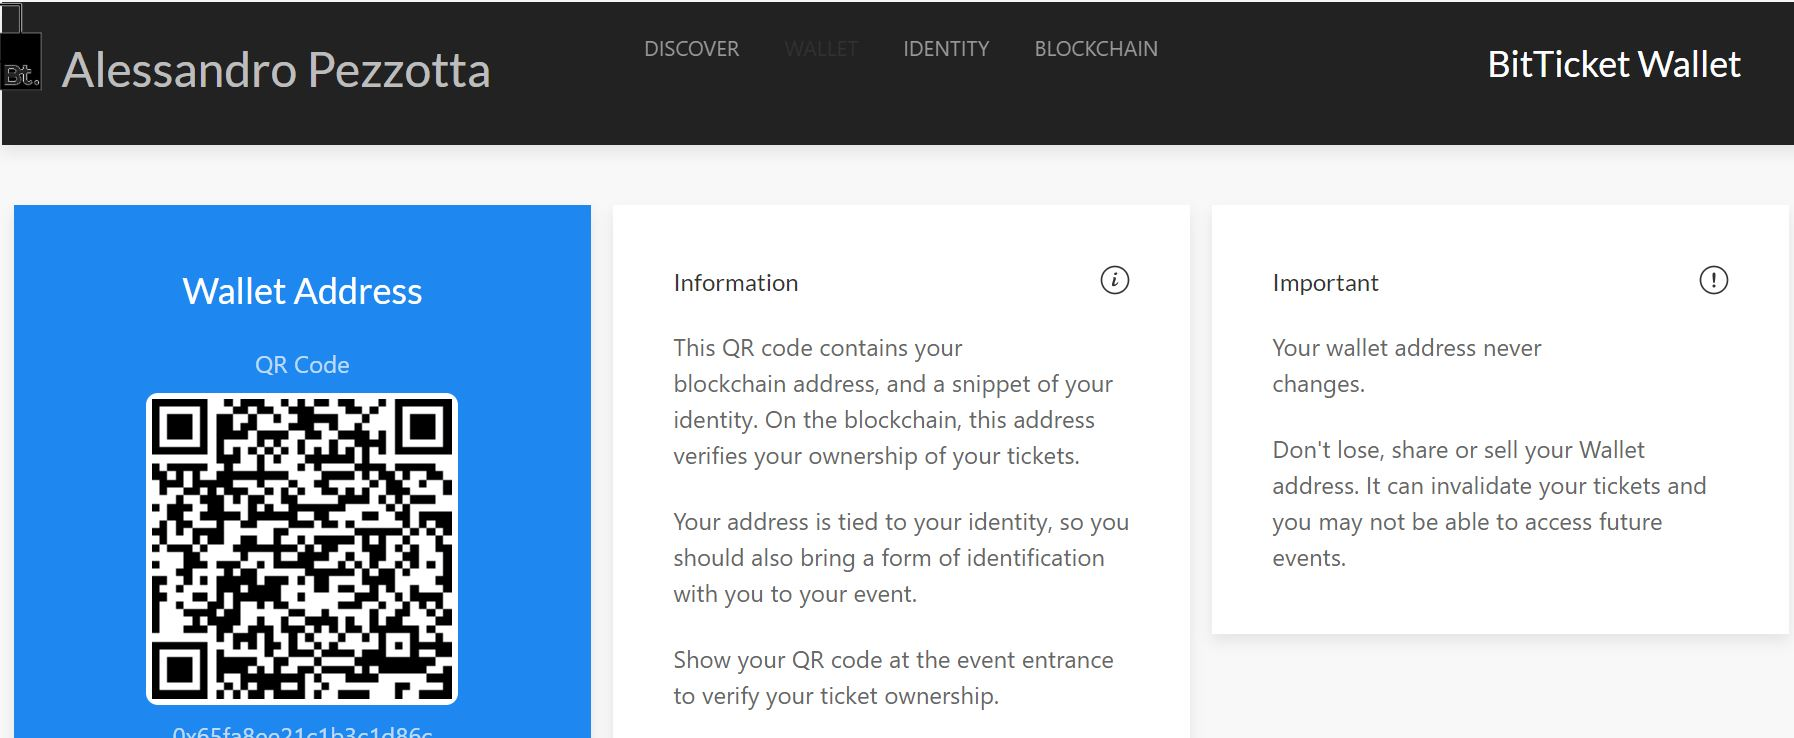
\includegraphics[width=0.68\textwidth]{chapter3/immagini/bitticket_bc}
	\caption{Indirizzo sulla blockchain BitTicket}
	\label{blockchain}
\end{figure}
Ogni biglietto è univocamente associato all'indirizzo sulla blockchain, e pertanto ogni passaggio di proprietà andrà documentato, in modo che il titolo di accesso cambi proprietario e indirizzo della persona che parteciperà all'evento. 
%\subsubsection{} si può fottere la blockchain?
%\subsection{ShieldSquare} wait for them to answer the e-mail (LOL)
